\documentclass[border=10pt]{standalone}

\usepackage{tikz}
\usepackage{tikzsymbols}
\usetikzlibrary{calc,patterns,shapes.geometric}

\def\centerarc[#1](#2)(#3:#4:#5){\draw[#1] ($(#2)+({#5*cos(#3)},{#5*sin(#3)})$) arc (#3:#4:#5);}

\begin{document}
	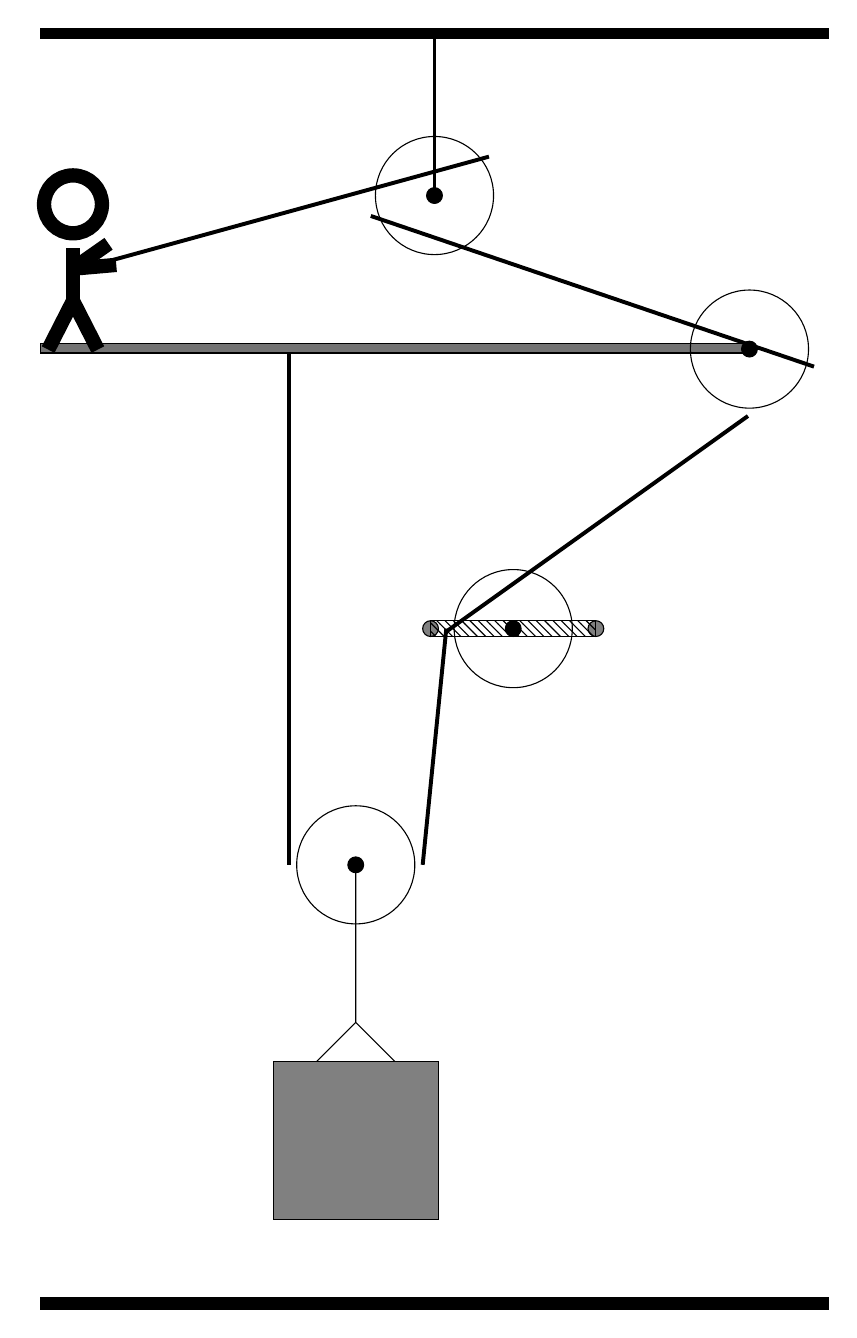
\begin{tikzpicture}
		%%%%% START %%%%%
		\draw[fill=black] (-2, 14) rectangle (8, 14.125);
		
		\draw[fill=black!55] (-2, 10) rectangle (7, 10.125);
		
		\draw (2, 3.5) circle (0.75);
		\draw[fill=black] (2, 3.5) circle (0.1);
		
		\draw (7, 10.05) circle (0.75);
		\draw[fill=black] (7, 10.05) circle (0.1);
		
		\draw[fill=white](4, 6.5) circle (0.75);
		\draw[fill=black] (4, 6.5) circle (0.1);
		\draw[fill=black!50] (2.95, 6.5) circle (0.1);
		\draw[fill=black!50] (5.05, 6.5) circle (0.1);
		\draw[pattern=north west lines, pattern color=black] (2.95, 6.6) rectangle (5.05, 6.4);
		
		\draw (3, 12) circle (0.75);
		\draw[fill=black] (3, 12) circle (0.1);
		\draw[line width=0.5mm] (3, 12) -- (3, 14);
		
		\draw (2, 3.5) -- (2, 1.5) -- (1.5, 1.0) -- (2.5, 1.0) -- (2, 1.5);
		\draw[fill=black!50] (0.95, 1.0) rectangle (3.05, -1.0);
		
		\draw[line width=0.5mm] (1.15, 10) -- (1.15, 3.5);
		\centerarc[line width=0.5mm](2, 3.5)(180:360:0.85);
		\draw[line width=0.5mm](2.85, 3.5) -- (3.15, 6.5);
		\centerarc[line width=0.5mm](4, 6.5)(110:180:0.85);
		\draw[line width=0.5mm](3.151, 6.463) -- (6.981, 9.2);
		\centerarc[line width=0.5mm](7, 10.05)(-60:50:0.85);
		\draw[line width=0.5mm](7.82, 9.827) -- (2.191, 11.741);
		\centerarc[line width=0.5mm](3, 12)(60:120:0.85);
		\draw[line width=0.5mm](3.692, 12.494) -- (-1.2, 11.15);
		
		\node at (-1.5, 11.15) {\Strichmaxerl[10][-175][35]};
		
		\draw[fill=black] (-2, -2) rectangle (8, -2.15);
		%%%%% END %%%%%
	\end{tikzpicture}
\end{document}